\chapter{Porte logiche in tecnologia c-MOS}
	
	I principali componenti attuali utilizzati nei dispositivi digitali sono realizzati mediante l'implementazione su chip di transistor opportunamente connessi. Come visto i mosfet sono degli oggetti che sono intrinsecamente analogici, tuttavia il loro principio di funzionamento gli rende altamente adatti a realizzare funzioni digitali.
	
	A livello digitale infatti i transistor possono essere considerati come degli interruttori che permettono o negano il passaggio di corrente tra i propri terminali. Considerando infatti la caratteristica statica dell'n-mos (figura \ref{fig:intro:nmos-carattstatica}, pagina \pageref{fig:intro:nmos-carattstatica}) è possibile osservare che se si pone una tensione di gate $V_g$ nulla (più in generale inferiore della tensione di soglia $\Vtn$) il dispositivo non permette il passaggio di corrente ai suoi capi (indipendentemente dalla tensione differenziale $V_{ds}$ applicata); usciti dalla fascia di interdizione è possibile osservare invece che, in funzione della tensione $\Vgs$, è possibile avere un passaggio di corrente attraverso i terminali del mosfet.\\
	Dualmente si dimostra che se la tensione $V_g$ applicata al gate di un transitor p-mos è elevata (tale per cui la differenza $|V_{ds}|$ sia minore della tensione di soglia $|V_{tp}|$) allora il componente risulta interdetto e non permette il passaggio di corrente.
	
	Questa peculiarità nel funzionamento duale dei componenti è particolarmente utile nelle implementazioni digitali dove in generale si considerano i segnali di tensione (intrinsecamente analogici) come dei segnali binari di valore basso (0) associato alla tensione di massa e valore alto (1) associato alla tensione di alimentazione $V_{dd}$.
	
	Lo scopo di questo capito è dunque quello di osservare e rappresentare le porte logiche che compongono ogni circuito combinatorio di un dispositivo tecnologico.

\section{Not gate}
	
	La porta logica più semplice da realizzare, composta da solamente due transistori, è il \textit{gate not}, ossia l'invertitore logico che realizza la seguente tabella di verità:
	\begin{center}
	\begin{tabular}{c | c}
			input & output \\ \hline
			0 & 1 \\ 1 & 0
	\end{tabular}
	\end{center}
	
	L'implementazione circuitale di questa porta è mostrata in figura \ref{fig:not:schematico} ed è realizzata ponendo in serie un p-mos con un n-mos: l'ingresso $V_{in}$ del segnale digitale viene applicato ad entrambi i gate dei transistor, mentre il segnale in uscita $V_{out}$ viene rilevato nel collegamento tra i due mosfet.
	
	\begin{figure}[bht]
		\centering
		\begin{subfigure}{0.48\linewidth}
			\centering
			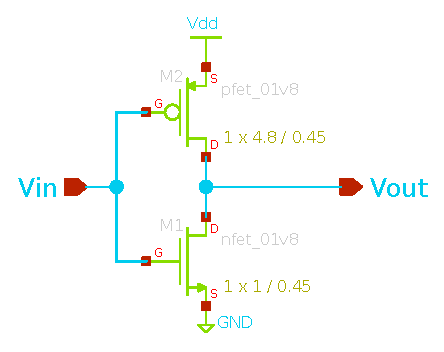
\includegraphics[width=5cm]{Immagini/not-gate.eps} \caption{}			
		\end{subfigure}
		\begin{subfigure}{0.48\linewidth}
			\centering
			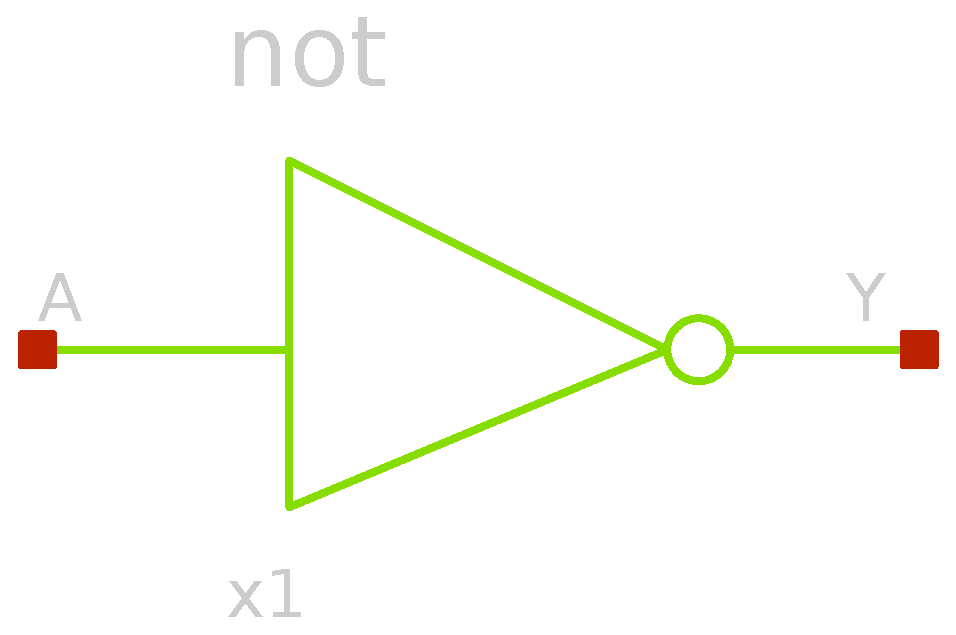
\includegraphics[width=2.5cm]{Immagini/not-gate-simple.eps} \caption{}			
		\end{subfigure}
		\caption{implementazione di un invertitore logico in tecnologia c-mos (a) e relativa rappresentazione semplificata per circuiti logici (b).} 
		\label{fig:not:schematico}
	\end{figure}
	
	Per comprendere il funzionamento del sistema è sufficiente considerare la prima legge di Kirchhoff bilanciando la corrente al nodo rispetto alla quale si rileva il segnale in uscita $\Vout$ che si traduce nell'eguagliare le correnti generate dai due transistor:
	\[ I_n = I_p \]
	
	A questo punto è possibile procedere con l'analisi del circuito per casi:
	\begin{itemize}
		\item nel caso in cui la tensione in ingresso sia bassa ($V_{in} = 0$) allora l'n-mos risulterebbe essere interdetto ($I_n = 0$), mentre il p-mos è posto in regime di saturazione. L'unica condizione che permette al p-mos di non far scorrere attraverso i suoi terminali è quella per cui la tensione differenziale $V_{ds}$ sia nulla: questo porta dunque ad affermare che
		\[ V_d = V_s \qquad \Rightarrow \qquad V_{out} = V_{dd} \]
		
		\item analogamente nel caso in cui l'ingresso si trovi ad una tensione in ingresso alta ($V_{in} = V_{dd}$), il p-mos risulterà interdetto, non permettendo il passaggio di alcuna corrente. Condizione necessaria affinché anche l'n-mos annulli la corrente attraverso i suoi terminali è che la tensione differenziale $V_{ds}$ sia nulla, e dunque
		\[ V_{out} = 0 \]
	\end{itemize} 
	
	In figura \ref{fig:not:carattstatica} è possibile invece osservare la caratteristica statica analogica realizzata dal dispositivo.
	
	\begin{figure}[H]
		\centering
		% GNUPLOT: LaTeX picture with Postscript
\begingroup
  \makeatletter
  \providecommand\color[2][]{%
    \GenericError{(gnuplot) \space\space\space\@spaces}{%
      Package color not loaded in conjunction with
      terminal option `colourtext'%
    }{See the gnuplot documentation for explanation.%
    }{Either use 'blacktext' in gnuplot or load the package
      color.sty in LaTeX.}%
    \renewcommand\color[2][]{}%
  }%
  \providecommand\includegraphics[2][]{%
    \GenericError{(gnuplot) \space\space\space\@spaces}{%
      Package graphicx or graphics not loaded%
    }{See the gnuplot documentation for explanation.%
    }{The gnuplot epslatex terminal needs graphicx.sty or graphics.sty.}%
    \renewcommand\includegraphics[2][]{}%
  }%
  \providecommand\rotatebox[2]{#2}%
  \@ifundefined{ifGPcolor}{%
    \newif\ifGPcolor
    \GPcolorfalse
  }{}%
  \@ifundefined{ifGPblacktext}{%
    \newif\ifGPblacktext
    \GPblacktexttrue
  }{}%
  % define a \g@addto@macro without @ in the name:
  \let\gplgaddtomacro\g@addto@macro
  % define empty templates for all commands taking text:
  \gdef\gplbacktext{}%
  \gdef\gplfronttext{}%
  \makeatother
  \ifGPblacktext
    % no textcolor at all
    \def\colorrgb#1{}%
    \def\colorgray#1{}%
  \else
    % gray or color?
    \ifGPcolor
      \def\colorrgb#1{\color[rgb]{#1}}%
      \def\colorgray#1{\color[gray]{#1}}%
      \expandafter\def\csname LTw\endcsname{\color{white}}%
      \expandafter\def\csname LTb\endcsname{\color{black}}%
      \expandafter\def\csname LTa\endcsname{\color{black}}%
      \expandafter\def\csname LT0\endcsname{\color[rgb]{1,0,0}}%
      \expandafter\def\csname LT1\endcsname{\color[rgb]{0,1,0}}%
      \expandafter\def\csname LT2\endcsname{\color[rgb]{0,0,1}}%
      \expandafter\def\csname LT3\endcsname{\color[rgb]{1,0,1}}%
      \expandafter\def\csname LT4\endcsname{\color[rgb]{0,1,1}}%
      \expandafter\def\csname LT5\endcsname{\color[rgb]{1,1,0}}%
      \expandafter\def\csname LT6\endcsname{\color[rgb]{0,0,0}}%
      \expandafter\def\csname LT7\endcsname{\color[rgb]{1,0.3,0}}%
      \expandafter\def\csname LT8\endcsname{\color[rgb]{0.5,0.5,0.5}}%
    \else
      % gray
      \def\colorrgb#1{\color{black}}%
      \def\colorgray#1{\color[gray]{#1}}%
      \expandafter\def\csname LTw\endcsname{\color{white}}%
      \expandafter\def\csname LTb\endcsname{\color{black}}%
      \expandafter\def\csname LTa\endcsname{\color{black}}%
      \expandafter\def\csname LT0\endcsname{\color{black}}%
      \expandafter\def\csname LT1\endcsname{\color{black}}%
      \expandafter\def\csname LT2\endcsname{\color{black}}%
      \expandafter\def\csname LT3\endcsname{\color{black}}%
      \expandafter\def\csname LT4\endcsname{\color{black}}%
      \expandafter\def\csname LT5\endcsname{\color{black}}%
      \expandafter\def\csname LT6\endcsname{\color{black}}%
      \expandafter\def\csname LT7\endcsname{\color{black}}%
      \expandafter\def\csname LT8\endcsname{\color{black}}%
    \fi
  \fi
    \setlength{\unitlength}{0.0500bp}%
    \ifx\gptboxheight\undefined%
      \newlength{\gptboxheight}%
      \newlength{\gptboxwidth}%
      \newsavebox{\gptboxtext}%
    \fi%
    \setlength{\fboxrule}{0.5pt}%
    \setlength{\fboxsep}{1pt}%
\begin{picture}(4250.00,2154.00)%
    \gplgaddtomacro\gplbacktext{%
      \csname LTb\endcsname%%
      \put(814,704){\makebox(0,0)[r]{\strut{}$0$}}%
      \csname LTb\endcsname%%
      \put(814,909){\makebox(0,0)[r]{\strut{}$0.3$}}%
      \csname LTb\endcsname%%
      \put(814,1114){\makebox(0,0)[r]{\strut{}$0.6$}}%
      \csname LTb\endcsname%%
      \put(814,1319){\makebox(0,0)[r]{\strut{}$0.9$}}%
      \csname LTb\endcsname%%
      \put(814,1523){\makebox(0,0)[r]{\strut{}$1.2$}}%
      \csname LTb\endcsname%%
      \put(814,1728){\makebox(0,0)[r]{\strut{}$1.5$}}%
      \csname LTb\endcsname%%
      \put(814,1933){\makebox(0,0)[r]{\strut{}$1.8$}}%
      \csname LTb\endcsname%%
      \put(946,484){\makebox(0,0){\strut{}$0$}}%
      \csname LTb\endcsname%%
      \put(1431,484){\makebox(0,0){\strut{}$0.3$}}%
      \csname LTb\endcsname%%
      \put(1915,484){\makebox(0,0){\strut{}$0.6$}}%
      \csname LTb\endcsname%%
      \put(2400,484){\makebox(0,0){\strut{}$0.9$}}%
      \csname LTb\endcsname%%
      \put(2884,484){\makebox(0,0){\strut{}$1.2$}}%
      \csname LTb\endcsname%%
      \put(3369,484){\makebox(0,0){\strut{}$1.5$}}%
      \csname LTb\endcsname%%
      \put(3853,484){\makebox(0,0){\strut{}$1.8$}}%
    }%
    \gplgaddtomacro\gplfronttext{%
      \csname LTb\endcsname%%
      \put(209,1318){\rotatebox{-270}{\makebox(0,0){\strut{}$V_{out}$ $[V]$}}}%
      \put(2399,154){\makebox(0,0){\strut{}$V_{in}$ $[V]$}}%
      \csname LTb\endcsname%%
      \put(2399,6582){\makebox(0,0){\strut{}}}%
    }%
    \gplbacktext
    \put(0,0){\includegraphics[width={212.50bp},height={107.70bp}]{Immagini/not_caratt}}%
    \gplfronttext
  \end{picture}%
\endgroup


		\caption{funzione di trasferimento statica dell'invertitore logico di figura \ref{fig:not:schematico}.}
		\label{fig:not:carattstatica}
	\end{figure}

	L'implementazione delle porte logiche in tecnologia c-mos è caratterizzata da una forte immunità al rumore. I transistor implementati infatti, alimentati ad una tensione di $1.8V$, permettono di avere una tensione $V_{ilmax}$ pari a circa $0.6V$ e $V_{ihmin} = 1.2V$: questo significa che il segnale in uscita da una porta logica a valle può acquisire fino a $0.6V$ di rumore senza inficiare sul corretto funzionamento del circuito.
	
	\subsection*{Caratteristiche dinamiche}
		
		Nota la caratteristica statica del circuito logico, di rilevante interesse pratico è l'analisi dinamica del circuito, in quanto permetterà di stabilire a regime quale sarà la massima frequenza di commutazione della porta logica.
		
		\begin{figure}[bht]
			\centering
			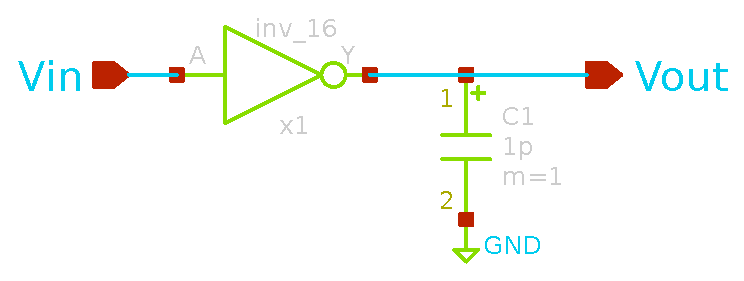
\includegraphics[width=5cm]{Immagini/not-gate-carico}
			\caption{schema circuitale di riferimento per l'analisi della risposta dinamica di un invertitore logico che deve pilotare un circuito a valle modellato da una capacità di $100fF$.}
			\label{fig:not:dinamica-schema}
		\end{figure}
		
		A tale fine è necessario considerare un'invertitore, come in figura \ref{fig:not:dinamica-schema}, che pilota un circuito a valle che può essere modellato come una capacità (in questo caso di valore nominale di $100fF$).
	
		\begin{figure}[bht]
			\centering
			% GNUPLOT: LaTeX picture with Postscript
\begingroup
  \makeatletter
  \providecommand\color[2][]{%
    \GenericError{(gnuplot) \space\space\space\@spaces}{%
      Package color not loaded in conjunction with
      terminal option `colourtext'%
    }{See the gnuplot documentation for explanation.%
    }{Either use 'blacktext' in gnuplot or load the package
      color.sty in LaTeX.}%
    \renewcommand\color[2][]{}%
  }%
  \providecommand\includegraphics[2][]{%
    \GenericError{(gnuplot) \space\space\space\@spaces}{%
      Package graphicx or graphics not loaded%
    }{See the gnuplot documentation for explanation.%
    }{The gnuplot epslatex terminal needs graphicx.sty or graphics.sty.}%
    \renewcommand\includegraphics[2][]{}%
  }%
  \providecommand\rotatebox[2]{#2}%
  \@ifundefined{ifGPcolor}{%
    \newif\ifGPcolor
    \GPcolorfalse
  }{}%
  \@ifundefined{ifGPblacktext}{%
    \newif\ifGPblacktext
    \GPblacktexttrue
  }{}%
  % define a \g@addto@macro without @ in the name:
  \let\gplgaddtomacro\g@addto@macro
  % define empty templates for all commands taking text:
  \gdef\gplbacktext{}%
  \gdef\gplfronttext{}%
  \makeatother
  \ifGPblacktext
    % no textcolor at all
    \def\colorrgb#1{}%
    \def\colorgray#1{}%
  \else
    % gray or color?
    \ifGPcolor
      \def\colorrgb#1{\color[rgb]{#1}}%
      \def\colorgray#1{\color[gray]{#1}}%
      \expandafter\def\csname LTw\endcsname{\color{white}}%
      \expandafter\def\csname LTb\endcsname{\color{black}}%
      \expandafter\def\csname LTa\endcsname{\color{black}}%
      \expandafter\def\csname LT0\endcsname{\color[rgb]{1,0,0}}%
      \expandafter\def\csname LT1\endcsname{\color[rgb]{0,1,0}}%
      \expandafter\def\csname LT2\endcsname{\color[rgb]{0,0,1}}%
      \expandafter\def\csname LT3\endcsname{\color[rgb]{1,0,1}}%
      \expandafter\def\csname LT4\endcsname{\color[rgb]{0,1,1}}%
      \expandafter\def\csname LT5\endcsname{\color[rgb]{1,1,0}}%
      \expandafter\def\csname LT6\endcsname{\color[rgb]{0,0,0}}%
      \expandafter\def\csname LT7\endcsname{\color[rgb]{1,0.3,0}}%
      \expandafter\def\csname LT8\endcsname{\color[rgb]{0.5,0.5,0.5}}%
    \else
      % gray
      \def\colorrgb#1{\color{black}}%
      \def\colorgray#1{\color[gray]{#1}}%
      \expandafter\def\csname LTw\endcsname{\color{white}}%
      \expandafter\def\csname LTb\endcsname{\color{black}}%
      \expandafter\def\csname LTa\endcsname{\color{black}}%
      \expandafter\def\csname LT0\endcsname{\color{black}}%
      \expandafter\def\csname LT1\endcsname{\color{black}}%
      \expandafter\def\csname LT2\endcsname{\color{black}}%
      \expandafter\def\csname LT3\endcsname{\color{black}}%
      \expandafter\def\csname LT4\endcsname{\color{black}}%
      \expandafter\def\csname LT5\endcsname{\color{black}}%
      \expandafter\def\csname LT6\endcsname{\color{black}}%
      \expandafter\def\csname LT7\endcsname{\color{black}}%
      \expandafter\def\csname LT8\endcsname{\color{black}}%
    \fi
  \fi
    \setlength{\unitlength}{0.0500bp}%
    \ifx\gptboxheight\undefined%
      \newlength{\gptboxheight}%
      \newlength{\gptboxwidth}%
      \newsavebox{\gptboxtext}%
    \fi%
    \setlength{\fboxrule}{0.5pt}%
    \setlength{\fboxsep}{1pt}%
\begin{picture}(5668.00,3400.00)%
    \gplgaddtomacro\gplbacktext{%
      \csname LTb\endcsname%%
      \put(434,2067){\makebox(0,0)[r]{\strut{}$0$}}%
      \csname LTb\endcsname%%
      \put(434,2456){\makebox(0,0)[r]{\strut{}$0.6$}}%
      \csname LTb\endcsname%%
      \put(434,2846){\makebox(0,0)[r]{\strut{}$1.2$}}%
      \csname LTb\endcsname%%
      \put(434,3235){\makebox(0,0)[r]{\strut{}$1.8$}}%
      \csname LTb\endcsname%%
      \put(566,1717){\makebox(0,0){\strut{}}}%
      \csname LTb\endcsname%%
      \put(1369,1717){\makebox(0,0){\strut{}}}%
      \csname LTb\endcsname%%
      \put(2172,1717){\makebox(0,0){\strut{}}}%
      \csname LTb\endcsname%%
      \put(2975,1717){\makebox(0,0){\strut{}}}%
      \csname LTb\endcsname%%
      \put(3777,1717){\makebox(0,0){\strut{}}}%
      \csname LTb\endcsname%%
      \put(4580,1717){\makebox(0,0){\strut{}}}%
      \csname LTb\endcsname%%
      \put(5383,1717){\makebox(0,0){\strut{}}}%
    }%
    \gplgaddtomacro\gplfronttext{%
      \csname LTb\endcsname%%
      \put(-171,2651){\rotatebox{-270}{\makebox(0,0){\strut{}$V_{out}$ $[V]$}}}%
      \put(2974,1651){\makebox(0,0){\strut{}}}%
    }%
    \gplgaddtomacro\gplbacktext{%
      \csname LTb\endcsname%%
      \put(434,640){\makebox(0,0)[r]{\strut{}$0$}}%
      \csname LTb\endcsname%%
      \put(434,1029){\makebox(0,0)[r]{\strut{}$0.6$}}%
      \csname LTb\endcsname%%
      \put(434,1418){\makebox(0,0)[r]{\strut{}$1.2$}}%
      \csname LTb\endcsname%%
      \put(434,1807){\makebox(0,0)[r]{\strut{}$1.8$}}%
      \csname LTb\endcsname%%
      \put(566,290){\makebox(0,0){\strut{}0}}%
      \csname LTb\endcsname%%
      \put(1369,290){\makebox(0,0){\strut{}0.5}}%
      \csname LTb\endcsname%%
      \put(2172,290){\makebox(0,0){\strut{}1}}%
      \csname LTb\endcsname%%
      \put(2975,290){\makebox(0,0){\strut{}1.5}}%
      \csname LTb\endcsname%%
      \put(3777,290){\makebox(0,0){\strut{}2}}%
      \csname LTb\endcsname%%
      \put(4580,290){\makebox(0,0){\strut{}2.5}}%
      \csname LTb\endcsname%%
      \put(5383,290){\makebox(0,0){\strut{}3}}%
    }%
    \gplgaddtomacro\gplfronttext{%
      \csname LTb\endcsname%%
      \put(-171,1223){\rotatebox{-270}{\makebox(0,0){\strut{}$V_{in}$ $[V]$}}}%
      \put(2974,-40){\makebox(0,0){\strut{}tempo $[ns]$}}%
    }%
    \gplbacktext
    \put(0,0){\includegraphics[width={283.40bp},height={170.00bp}]{Immagini/not-dinamica}}%
    \gplfronttext
  \end{picture}%
\endgroup


			\caption{risposta dell'invertitore logico (in figura \ref{fig:not:dinamica-schema}) ad un'onda quadra in ingresso di periodo $2ns$.}
			\label{fig:not:dinamica}
		\end{figure}
		
		In figura \ref{fig:not:dinamica} è possibile leggere la risposta dell'invertitore ad un'onda quadra in ingresso. Si osserva che un transitorio (associato in particolare alla commutazione dell'ingresso da basso a alto) è più veloce rispetto alla commutazione inversa: questo è dovuto all'assimetricità del comportamento dei transistor a drogaggio diverso. Infatti dall'analisi della caratteristica statica dei circuiti l'n-mos permette, a parità di rapporto $W/L$, di far scorrere attraverso i suoi terminali una quantità di corrente maggiore (per via della più elevata conducibilità intrinseca), rendendo più efficiente la polarizzazione della capacità di carico.
		
		Il valore di capacità di scelto è sufficientemente basso e ci permette di valutare dei parametri fondamentali per la risposta dinamica della porta logica quale i ritardi di propagazione dei segnali, ossia il tempo che intercorre tra la commutazione dell'ingresso e la rispettiva variazione dell'uscita. Questo parametro può essere valutato singolarmente sia per una variazione dell'ingresso da alto a basso $\tau_{hl}$, ma anche per lo stesso che passa da basso a alto $\tau_{lh}$ (in questo caso i tempi sono calcolati al $95\%$ dell'escursione di tensione):
		\[ \tau_{lh} = 68ps \qquad \tau_{hl} = 217ps  \] 



\section{Nor gate}
	La porta logica \textit{nor}, coincidente con la negazione del gate \textit{or}, è un gate che, insieme al \textit{nand}, costituisce un \textit{gate universale}, ossia in grado di realizzare, tramite delle opportune interconnessioni, tutte le funzioni logiche digitali. Tale porta a due (o più ingressi) rispetta la seguente tabella di verità:
	\begin{center}
		\begin{tabular}{c c | c}
			$V_{in,1}$ & $V_{in,2}$ & $V_{out}$ \\ \hline
			0 & 0 & 1 \\
			0 & 1 & 0 \\
			1 & 0 & 0 \\
			1 & 1 & 0 \\
		\end{tabular}
	\end{center}
	Si osserva dunque che tale porta logica determina un'uscita alta solamente se tutti i suoi ingressi sono bassi, mentre in tutti gli altri casi l'uscita è bassa.
	
	\begin{figure}[bht]
		
		\caption{implementazione della porta logica nor in tecnologia c-mos (a) e la relativa rappresentazione schematica (b).}
		\label{fig:nor:schematico}
	\end{figure}

	In figura \ref{fig:nor:schematico} è dunque possibile osservare un'implementazione della porta logica nand in tecnologia c-mos.\\
	Tale circuito può essere analizzando le possibili combinazioni di ingresso presenti nella tabella di verità:
	\begin{itemize}
		\item nel caso in cui entrambi gli ingressi si trovano ad un valore basso (prima riga della tabella di verità), allora risultano interdetti i transistor a substrato n, mentre la rete di pull-up composta dai due p-mos in serie risulta essere attiva. L'unico modo per garantire corrente nulla in uscita dal circuito è quello di avere tensione differenziale $V_{ds}$ dei p-mos nulla, ossia nel caso in cui $V_{out} = V_{dd}$, verificando la tabella di verità;
		
		\item in tutti gli altri casi in cui almeno un segnale si trova in uno stato di tensione alto si osserva che la rete di pull-up sarà sicuramente interdetta (il p-mos associato all'ingresso alto non permette infatti passaggio di corrente), e dunque la tensione in uscita sarà determinata dalla rete di pull-down degli n-mos che risulteranno attivi. Sempre per imposizione della condizione di corrente nulla al nodo d'uscita si ottiene che la tensione differenziale $V_{ds}$ degli n-mos deve essere nulla e dunque $V_{out} = 0$.
	\end{itemize}
